\documentclass[legalpaper,10pt]{article}
\usepackage[left=1.50cm, right=2.0cm, top=2.00cm, bottom=1.00cm]{geometry}
\usepackage{multicol}
\usepackage{graphicx}
\usepackage{amsmath,amsfonts,amssymb}

\setlength{\columnsep}{1cm}
\title{\textbf{\LARGE{Optics}} \\ Interference,  Diffraction, Polarization}
\author{prepared by Shanku}

\begin{document}
	\maketitle
	\begin{multicols*}{2}
		
		\section*{Huygens Principal}
		According to Huygens, a light source in a \textit{homogeneous isotropic medium} sends out light in every direction \& these waves travel with equal velocity to carry energy with them to be transmitted in all directions.
		\begin{enumerate}
			\item {Every point on a given wavefront may be regarded as the source of a new disturbance, called \bf{secondary wavelets.}}
			\item The secondary wavelets(spherical) from each point spread out in all directions with the velocity of light.
			\item The envelope of these wavelets in the forward direction at any instance constitutes the new wave front at the instance.
		\end{enumerate}
		\paragraph{Wavefront-}defined as a \textit{surface} on which the phase of the disturbance is the same at any given instant of time. (two types = spherical /cylindrical)
		\paragraph{Huygens Principal can}
		\begin{itemize}
			\item Refraction \& reflection. Double Refraction in crystals.
			\item
		\end{itemize}
		\paragraph{Huygens Principal cannot}
		\begin{itemize}
			\item Geometrical shadow theory.
			\item Diffraction interference.
		\end{itemize}
		
		\subsection*{Path Difference vs Phase Difference}
		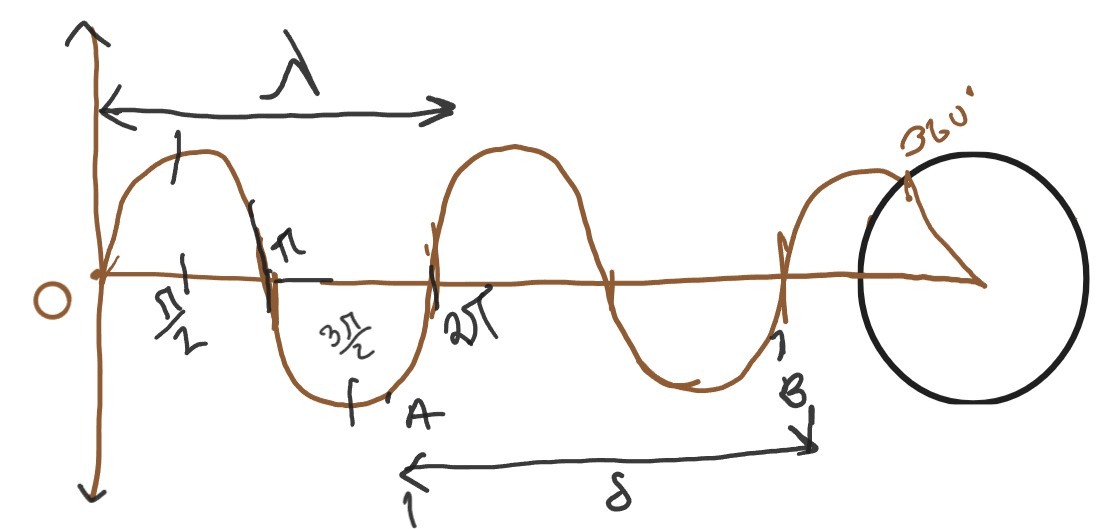
\includegraphics[width=7cm]{abc.png}
		Suppose 2 points $A\,and\,B$\par
		path difference $OB-OA=\delta$\par
		let, Phase difference $=\theta$\\
		we know if the difference between two waves equals to its wavelength($\lambda$) then $\theta=2\pi\,[360^{\circ}]$\par
		for path distance $\lambda$ phase diff $=2\pi$\par
		for path distance $\delta$ phase diff $=\dfrac{2\pi}{\lambda}\theta$\\
		\indent so, \(\mathbf{\boxed{\theta=2\pi\delta/\lambda }}\)
		
		\paragraph{Coherent Source:}the phase diff between the interfering waves must be zero or constant.
		
		\section*{Interference}
		\paragraph{Superposition}stats that.. the resultant disturbance of two or more waves acting on the same point simultaneously is the vector sum of the individual waves(disturbances).
		\begin{align*}
			\text{Let, }y_1=a\sin{\omega t}, & \text{ and } \,y_2=a\sin{(\omega t+\theta)}, \\
			\text{so, resultant will, }      & y=y_1+y_2
			\\= &a[\sin{\omega t}+\sin{(\omega t+\theta)}]
			\\= &2a \sin{(\omega t+\frac{\theta}{2}) \sin{\frac{\theta}{2}}}
			\\= &A \sin{(\omega t+\frac{\theta}{2})}
		\end{align*}
		\paragraph{Interference of light - the phenomenon where  \textit{monochromatic} light waves coming from two or more \textit{coherent sources}  Superimpose,  This leads to regions of constructive interference (brighter) and destructive interference (darker), creating an interference pattern.}
		
		\subsection*{Young's Double slit Experiment}
		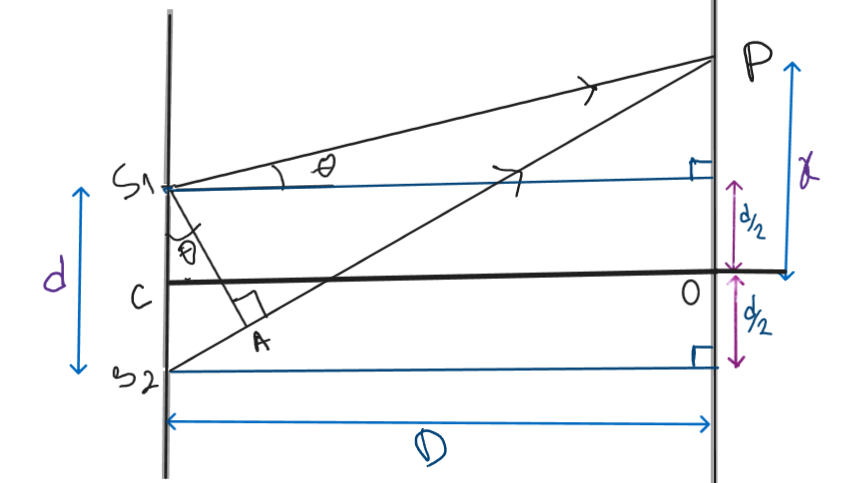
\includegraphics[width=9cm,height=4cm]{young1.png}\\
		\begin{math}
			\hspace*{1.5cm} l_1^2  =D^2+(x-d/2)^2
			\\\hspace*{1.5cm} l_2^2 =D^2+(x+d/2)^2
			\\\indent\text{  so, }(l_1+l_2)(l_1-l_2)=(x-d/2)^2 -(x+d/2)^2
			\\\indent\implies (l_1-l_2)\,2D=2xd
			\\\indent\implies l_1-l_2= path\, difference,\\
			\\\hspace*{3cm}\therefore \;\boxed{\bf{\delta=xd/D}}\\
		\end{math}
		% \pagebreak
		\\or, another way,\\
		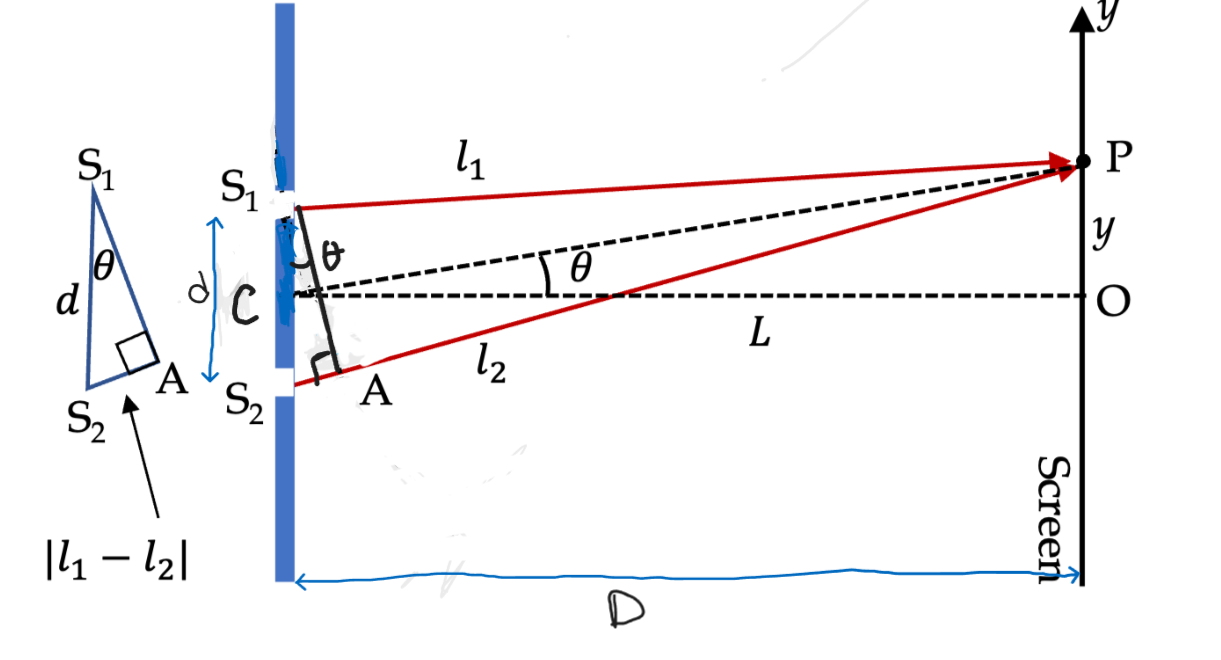
\includegraphics[width=9cm,height=4cm]{young2.png}\\
		\begin{math}
			\\\indent S_2A=\delta = S_1P-S_2P=l_1-l_2,\quad (D=CP)
			\\\indent\text{and in }\triangle S_1AS_2, \quad \sin{\theta}=S_2A/{S_1S_2}
			\\\indent\hspace*{2cm} \text{or,}\indent S_2A=\delta=d\sin{\theta}
			\\\indent P \,\& \,O \text{ are very close when, }  S_1P \approx S_2P \approx D
			\\\indent\text{as }[d<<D]\text{ and $y$ is very small}
			\\\indent\text{then, }\theta=\angle{S_2S_1A}=\angle{PCO}
			\\\therefore \quad \delta = d \sin\theta=\dfrac{dy}{PC}\approx \dfrac{dy}{D}\;  [if,\,S_1S_2=2d\implies \dfrac{2dy}{D} ]
		\end{math}\\
		\\\large\textbf{now}, \textit{from principle of interference we know, resultant amplitude }
		\\\indent \(A=2a\cos{\left(\dfrac{\theta}{2}\right)}=2a\cos{\left(\dfrac{2\pi\delta}{2\lambda}\right)}\)\\
		\\\indent \(\delta=\lambda\sigma/2\pi\)
		
		\subsubsection*{Conditions for sustained interference:}
		\begin{itemize}
			\item must be coherent(same $\lambda$ or $\theta$),\\so we \textbf{can't use two real sources} they can't be coherent.(also $a_1\ne a_2$)
			\item same frequency($f$) or wavelength($\lambda$).\\\textbf{so,} if we cover slits with different transparent color paper that's lead to $\lambda_a \ne \lambda_b$
			\item if Polarized, then must be in same state of Polarization
			\item medium matters cause in water,\\ \(\beta'=\dfrac{D{\lambda}'}{d} = \beta'=\dfrac{D}{d}\dfrac{\lambda}{\mu}\)\\ so, $\beta{'} < \beta$ ,means width will reduced.
		\end{itemize}
		\subsubsection*{Conditions for good observation:}
		\begin{itemize}
			\item \(d\) must be small,\\\textbf{but if \({d<\lambda}\)} then $\beta$ is extremely large, lead to an \textbf{uniform illumination} got \textbf{no visible fringes}. \([\beta\propto(\lambda/d)]\)
			\item \(D\) should be relatively large. \(\beta \varpropto  D \)
			\item Background should be darker.
		\end{itemize}
		\subsubsection*{Conditions for good  contrast:}
		\begin{itemize}
			\item amplitudes should be equal or very nearly equal \(I_{m} \propto (a_1 \pm a_2)^2\; \text{  so, }a_1 \approxeq a_2\)
			\item the sources must be narrow
			\item sources must be monochromatic or very nearly so.
		\end{itemize}
		\paragraph*{Conservation of energy in interference:}In case of constructive interference, $I=I_{max}$ and bright fringes are formed in the screen. Whereas in case of destructive interference, $I=I_{min}$, dark fringes are formed.
		\par This implies that in interference and diffraction pattern, the intensity of light is simply being redistributed \textbf{i.e. energy is only transferred from dark to bright fringe and no energy is created or destroyed in the process.}
		\begin{align*}
			I_\text{total} & = I_1 + I_2                             \\
			& = I_1 + I_2 + 2\sqrt{I_1 I_2}\ \cos\phi
		\end{align*}
		
		
		\section*{Diffraction}
		\textbf{The phenomenon of bending of light waves around obstacles or (aperture of sizes comparable with the wavelengths of light) \& resulting thereby in their spreading in \textit{Geometrical shadow} of the object is known as Diffraction.}
		\par It is a fundamental phenomenon in wave physics that occurs with all types of waves, including sound waves, electromagnetic waves (such as visible light, X-rays, and radio waves), and even matter waves (such as electrons and neutrons).\\
		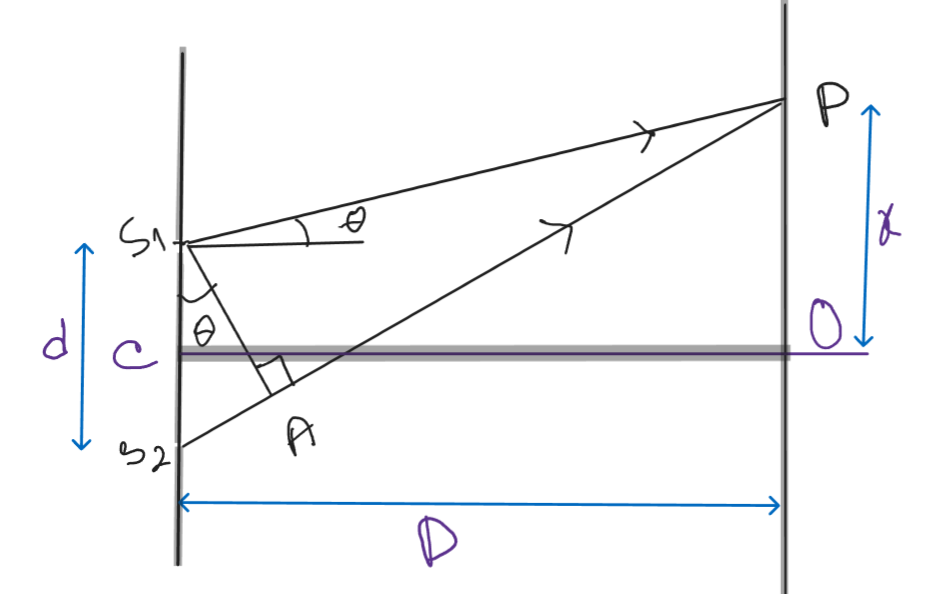
\includegraphics[width=9cm,height=4cm]{difraction.png}
		\begin{math}
			\\\indent\textit{path difference, }\delta=l_1-l_2,
			\\\indent\text{and in }\triangle S_1AS_2, \quad \sin{\phi}=S_2A/{S_1S_2}
			\\\indent\hspace*{2cm} \text{or, }\delta=d\sin{\phi}
			\\\indent\textit{so, phase difference, }\theta=\dfrac{2\pi}{\lambda}\delta=\dfrac{2\pi}{\lambda} a\sin{\phi}
		\end{math}
		\paragraph{\large The key aspects of diffraction are:}
		\begin{itemize}
			\item \textbf{Bending of waves around obstacles:} When waves encounter an obstacle or an edge, they tend to bend around it, rather than traveling in a straight line.
			\item \textbf{Spreading of waves through apertures:} When waves pass through a small opening or aperture, they spread out and diverge, rather than traveling in a straight beam.
			\item \textbf{Interference patterns:} The bending and spreading of waves can create interference patterns, where the waves constructively and destructively interfere with each other, leading to regions of higher and lower intensity.
		\end{itemize}
		\subsection*{Types of diffraction}
	\begin{description}
		\item[1. Fresnel type] the source and the screen \textit{(i.e. the point of observation)} or both are at finite distance from the obstacle or the aperture.
			\item[2. Fraunhofer type]  both source and screen are \textit{at $\infty$ distance }from each other.
		\end{description}
		
	\end{multicols*}
\end{document}
